%!TEX root = ../main.tex
%%%%%%%%%%%%%%%%%%%%%%%%%%%%%%%%%%
% Links:
%
% Difficulty: Companies: 
%%%%%%%%%%%%%%%%%%%%%%%%%%%%%%%%%%

\chapter{Binary Tree mirroring}
\label{ch:mirror_binary_tree}
\section*{Introduction}
Binary trees are one of the most taught and discussed data structures in computer science courses. A
binary tree is a tree-like data structure where each node has at most two children, which we refeer
to as right and left children. Trees have been used in computer science for a long time as a mean to
accessing data stored within the nodes that are usually arranged in some particular way such that
operations like searching for sorting can be performed more efficiently. Examples of such special
kind of trees are: 
\begin{itemize*}
	\item binary search tree,
	\item binary heap
\end{itemize*}

But binary trees are often also used to model data haveing an inherently bifurcating structure, where
the organization of data into left and right is part of the information we are representing\footnote{In such
case changing the arrangements of the node would change the meaning of the data.}.
A tree is recursive a data structure because you can think of it as either being:
\begin{itemize}
	\item an empty tree
	\item or a node having a binary tree as left and right children.
\end{itemize}
There are many recursive fundamental algorithms on trees described in the literature that built around this definition, 
and you can expect recursive solutions to questions about trees to be an effective tool during coding interviews.
The problem discussed in this chapter is about the manipulation of a binary tree into another binary tree
such that the latter is a mirror image of the former. As we will see this question is quite vague as it will be quite unclear what 
being a mirror really means and it will be imperative for you to clear this aspect up by asking relevant questions and 
creating a few examples cases (which we provide later in this chapter) that make clear to you what the interviewer is expecting. 

The tree definition that we will use thoroughout the chapter is shown in Listing \ref{list:binary_tree_definition}.
\lstinputlisting[language=c++, caption={Definition of the tree data structure using in Chapter \ref{ch:mirror_binary_tree}.},label=list:binary_tree_definition]{sources/mirror_binary_tree/binary_tree.h}

\section{Problem statement}
\begin{exercise}
	Write a function that given a binary tree, return mirror copy of it.

	\begin{example}
		\hfill \\
		Given the binary tree shown in Figure \ref{fig:mirro_binary_tree:example1} the function
		returns a tree like the one in Figure \ref{fig:mirro_binary_tree:example1_1}
		\label{ex:mirro_binary_tree:example1}.
	\end{example}

	\begin{example}
		\hfill \\
		Given the binary tree shown in Figure \ref{fig:mirro_binary_tree:example2} the function
		returns a tree like the one in Figure \ref{fig:mirro_binary_tree:example2_1}
		\label{ex:mirro_binary_tree:example2}
	\end{example}

	\begin{example}
		\hfill \\
		Given the binary tree shown in Figure \ref{fig:mirro_binary_tree:example3} the function
		returns a tree like the one in Figure \ref{fig:mirro_binary_tree:example3_1}
		\label{ex:mirro_binary_tree:example3}
	\end{example}
\end{exercise}


\begin{figure}
	\centering
	\begin{subfigure}[b]{0.25\textwidth}
	   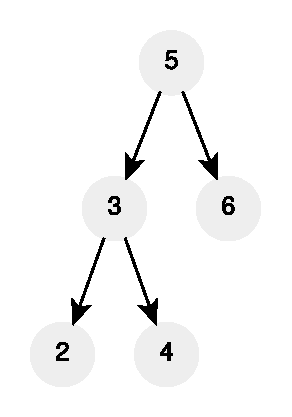
\includegraphics[]{sources/mirror_binary_tree/images/example1}
	   \caption{Input binary tree for the Example \ref{ex:mirro_binary_tree:example1}.}
	   \label{fig:mirro_binary_tree:example1}
	\end{subfigure}
	\hfill
	\begin{subfigure}[b]{0.4\textwidth}
	   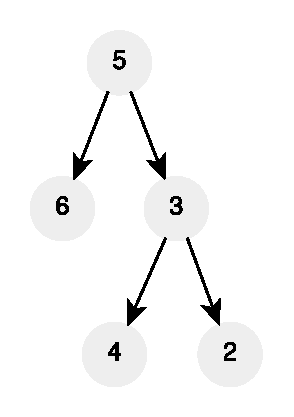
\includegraphics[]{sources/mirror_binary_tree/images/example1_1}
	   \caption{Output binary tree for the Example \ref{ex:mirro_binary_tree:example1}.}
	   \label{fig:mirro_binary_tree:example1_1}
	\end{subfigure}
	\centering
	\begin{subfigure}[b]{0.4\textwidth}
	   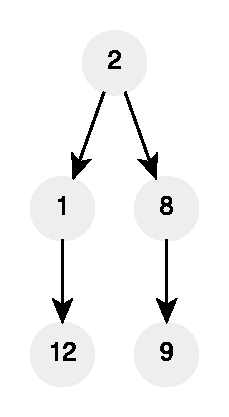
\includegraphics[]{sources/mirror_binary_tree/images/example2}
	   \caption{Input binary tree for the Example \ref{ex:mirro_binary_tree:example2}.}
	   \label{fig:mirro_binary_tree:example2}
	\end{subfigure}
	\hfill
	\begin{subfigure}[b]{0.4\textwidth}
	   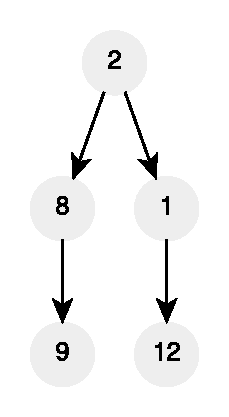
\includegraphics[]{sources/mirror_binary_tree/images/example2_1}
	   \caption{Output binary tree for the Example \ref{ex:mirro_binary_tree:example2}.}
	   \label{fig:mirro_binary_tree:example2_1}
	\end{subfigure}
	\centering

	 \caption[]{Input and output for Examples \ref{ex:mirro_binary_tree:example1} and
	 \ref{ex:mirro_binary_tree:example2}}
\end{figure}


\begin{figure}
	\centering
	\begin{subfigure}[b]{0.4\textwidth}
		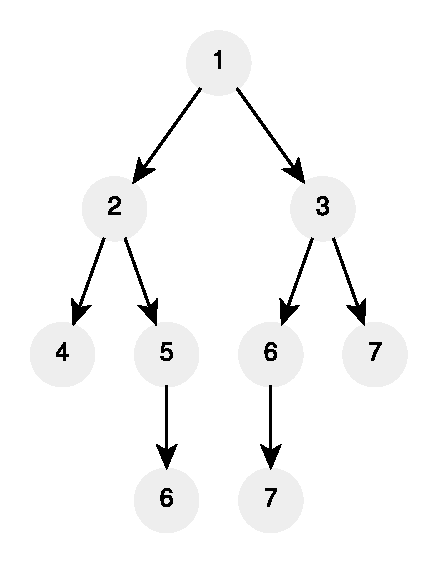
\includegraphics[]{sources/mirror_binary_tree/images/example3}
		\caption{Input binary tree for the Example \ref{ex:mirro_binary_tree:example3}.}
		\label{fig:mirro_binary_tree:example3}
	 \end{subfigure}
	 \hfill
	 \begin{subfigure}[b]{0.4\textwidth}
		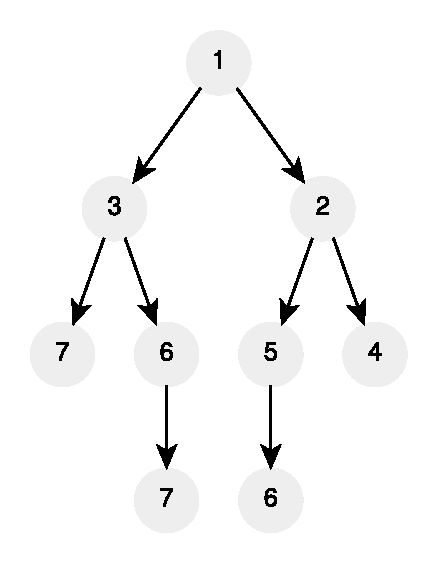
\includegraphics[]{sources/mirror_binary_tree/images/example3_1}
		\caption{Output binary tree for the Example \ref{ex:mirro_binary_tree:example3}.}
		\label{fig:mirro_binary_tree:example3_1}
	 \end{subfigure}
	 \caption[]{Input and output for Example \ref{ex:mirro_binary_tree:example3}}

\end{figure}



\section{Discussion}
\label{mirror_binary_tree:sec:discussion}
Let's start our discussion by trying to understand how a mirror copy of a tree really looks like. If
we have a tree $T$ rooted at node $n$ then its mirror image \rotatecharone{$T$} can be defined as
follows:
\begin{itemize}
	\item \textbf{if $n$ has no children:} return  $T$. See Figures \ref{fig:mirro_binary_tree:leaf}
	and \ref{fig:mirro_binary_tree:leaf_mirror}.
	\item \textbf{if $n$ has one only the left child $n_l$:}  return $T$ having as left child the a
	mirrored copy of $n_l$. See Figures \ref{fig:mirro_binary_tree:single_left} and
	\ref{fig:mirro_binary_tree:single_left_mirror}.
	\item \textbf{if $n$ has one only the left child $n_r$:}  return $T$ having as right child the a
	mirrored copy of $n_r$. See Figures \ref{fig:mirro_binary_tree:single_right} and
	\ref{fig:mirro_binary_tree:single_right_mirror}. 
	\item \textbf{if $n$ has both children:} return $T$ having as left child the mirrored copy of
	 its right child $n_r$ and, as right child the mirrored copy of its left child $n_l$.  See
	 Figures \ref{fig:mirro_binary_tree:tree_only_both_children} and
	 \ref{fig:mirro_binary_tree:tree_only_both_children_mirror}. Another example of this case can be
	 found in the node $5$ in the Example \ref{ex:mirro_binary_tree:example1} where its left and
	 right children are first mirrored individually and then swapped. 
\end{itemize}
This recursive definition can be refined into the following simple idea: In order to create the
mirror image of a tree $T$ rooted at $n$ we can first mirror its children individually and only
after swap them. Given that we can turn a tree into its mirror image all is  necessary is to first create a copy of the origin tree
and then mirror it (remember that the problem is asking to return a copy). 
Listing \ref{list:mirror_binary_tree1} shows a recursive implementation of such
idea.
\lstinputlisting[language=c++, caption={Solution to the problem of creating a mirror of a binary tree. Works by first creating a copy of the original tree and only then performing the mirroring.},label=list:mirror_binary_tree1]{sources/mirror_binary_tree/mirror_binary_tree_solution1.cpp}

The complexity of the code above is $O(n)$ where $n$ is the number of nodes in $T$.
However, despite it simplify the reasoning and the implementation,
splitting the copy and the mirroring steps, is not optimal as we need to traverse the whole tree twice. 
We can create the copy on the fly as we visit $T$ as shown in Listing \ref{list:mirror_binary_tree2}. 
This approach does not lower the asymptotic complexity but, it effectively means that 
we only need to traverse the original tree only once instead of twice. 

\lstinputlisting[language=c++, caption={Solution to the problem of creating a mirror of a binary tree. The copy and the mirroring are performed simultaneously while visiting $T$.},label=list:mirror_binary_tree2]{sources/mirror_binary_tree/mirror_binary_tree_solution2.cpp}

\begin{figure}
	\centering
	\begin{subfigure}[b]{0.4\textwidth}
		
\includegraphics[]{sources/mirror_binary_tree/images/leaf}
		\caption{Example of single node tree.}
		\label{fig:mirro_binary_tree:leaf}
	 \end{subfigure}
	 \hfill
	 \begin{subfigure}[b]{0.4\textwidth}
		
\includegraphics[]{sources/mirror_binary_tree/images/leaf}
		\caption{Mirror image of the tree in Figure \ref{fig:mirro_binary_tree:leaf}.}
		\label{fig:mirro_binary_tree:leaf_mirror}
	 \end{subfigure}
	 
	 \centering

	\begin{subfigure}[b]{0.4\textwidth}
		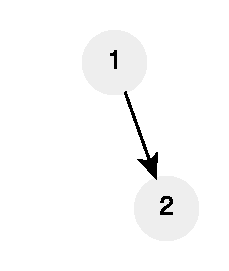
\includegraphics[]{sources/mirror_binary_tree/images/tree_only_right_child}
		\caption{Example of node with a single child: the right one.}
		\label{fig:mirro_binary_tree:single_right}
	 \end{subfigure}
	 \hfill
	 \begin{subfigure}[b]{0.4\textwidth}
		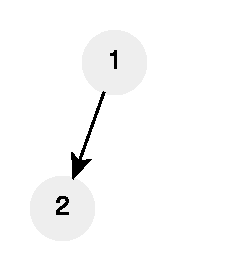
\includegraphics[]{sources/mirror_binary_tree/images/tree_only_right_child_mirror}
		\caption{Mirror image of the tree in Figure \ref{fig:mirro_binary_tree:single_right}.}
		\label{fig:mirro_binary_tree:single_right_mirror}
	 \end{subfigure}

	 \hfill
	 \begin{subfigure}[b]{0.4\textwidth}
		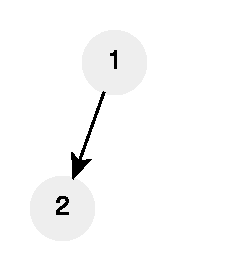
\includegraphics[]{sources/mirror_binary_tree/images/tree_only_right_child_mirror}
		\caption{Example of node with a single child: the left one.}
		\label{fig:mirro_binary_tree:single_left}
	 \end{subfigure}
	 \hfill
	 \begin{subfigure}[b]{0.4\textwidth}
		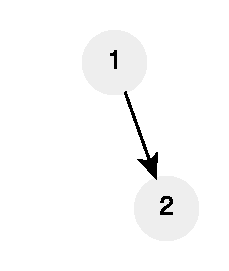
\includegraphics[]{sources/mirror_binary_tree/images/tree_only_right_child}
		\caption{Mirror image of the tree in Figure \ref{fig:mirro_binary_tree:single_right}.}
		\label{fig:mirro_binary_tree:single_left_mirror}
	 \end{subfigure}
	
	 \hfill

	 \begin{subfigure}[b]{0.4\textwidth}
		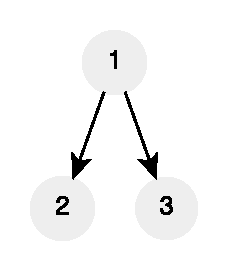
\includegraphics[]{sources/mirror_binary_tree/images/tree_only_both_children}
		\caption{Example of node with a single child: the left one.}
		\label{fig:mirro_binary_tree:tree_only_both_children}
	 \end{subfigure}
	 \hfill
	 \begin{subfigure}[b]{0.4\textwidth}
		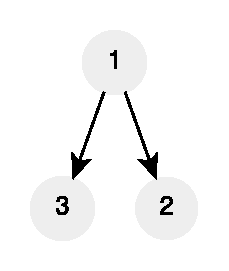
\includegraphics[]{sources/mirror_binary_tree/images/tree_only_both_children_mirror}
		\caption{Mirror image of the tree in Figure
		\ref{fig:mirro_binary_tree:tree_only_both_children}.}
		\label{fig:mirro_binary_tree:tree_only_both_children_mirror}
	 \end{subfigure}


\caption[]{Examples of various types of binary trees and their associated mirror images.}

\end{figure}
